% ================================================================
% Use the following if all authors are from the SAME institution
% ================================================================
\documentclass[accepted,single]{gipaper}

% use Times fonts
\usepackage{times}
% make sure English hyphenation rules, etc. loaded
\usepackage[english]{babel}
% permits inclusion of PNG, JPG, and PDF files under pdflatex
\usepackage{graphics}
\usepackage{graphicx}
\usepackage{caption}
% other packages
\usepackage{epsfig}
\usepackage{newalg}
\usepackage{floatflt}
\usepackage{array,amsmath,amssymb}

% a more flexible replacement for "verbatim" for typesetting pseudocode
\usepackage{alltt}
% gives automatic table of contents, permits setting PDF
% attributes of document.   Set page size in pdftex.cfg file;
% the "letterpaper" option to hyperref is unreliable...
\usepackage[
    pdftitle = "{Final Project Report}",
    pdfauthor = "{Your Name}"
]{hyperref}

% ================================================================

\title{Final Project Report \\
Smoke simulation in box-splines spaces\\
CPSC 503}

\newauthor{wd}{Estelle Altazin}{}

\affiliation{Department of Computer Science \\University of Calgary
\\\tt{ealtazin@cpsc.ucalgary.ca}}

% ================================================================
% Use the following if more than one author
% ================================================================
%
% \title{Final Project Report}
%
% \newauthor{wd}{Author One}{}
% \newauthor{se}{Someone Else}{}
% \newauthor{ya}{Yet Another}{}
% \newauthor{fa}{Fourth Author}{}
%
% \affiliation{Department of Computer Science \\University of Calgary
% \\\small{\{author1,author2,author2,author4\}@cpsc.ucalgary.ca} } }
%
% ================================================================
% The rest of the document follows.
% ================================================================

\abstract{Your text here...}

\begin{document}
\begin{keywords}
Your text here...\\
Your text here...\\
Your text here...\\
Your text here...\\
Your text here...\\
Your text here...\\
Your text here...\\
Your text here...\\
Your text here...\\
Your text here...\\
\end{keywords}


%###################################################################@@@@@######
\section{Introduction}

%==============================================================================
\subsection{Goal}

%++++++++++++++++++++++++++++++++++++++++++++++++++++++++++++++++++++++++++++++
\subsubsection{What did we try to do?}

The modeling and simulation of smoke is challenging and allows us to apprehend various mathematical methods specific to natural phenomenas or fluids simulation. The main goal of this project was to understand and implement all these methods in order to model and visualize smoke. This work was supposed to be done on both Cartesian and body-centered cubic (BCC) grids, so as to compare the results. The result is expected to be better on BCC grids.

%++++++++++++++++++++++++++++++++++++++++++++++++++++++++++++++++++++++++++++++
\subsubsection{Who would benefit?}

Smoke simulation could be use for special effects, or for games for example. More generally, this work is a contribution to the computer graphics community.

%==============================================================================
\subsection{Previous Work}

%++++++++++++++++++++++++++++++++++++++++++++++++++++++++++++++++++++++++++++++
\subsubsection{What related work have other people done?}
Fedkiw et al. \cite{Fedkiw:2001} have worked on Cartesian grids and obtained good results of smoke simulation. They design a model for smoke and gases, using numerical methods that are both fast and efficient. Solving the incompressible Euler equations to compute smoke's velocity, they then introduce a vorticity confinement term to model rolling features in order to make the smoke more realistic. Their model uses a finite difference approximation for the divergence and Laplacian operators with the goal of making the solution accurate at the grid points.
Alim \cite{alim:ms} worked on smoke simulation and describe the mathematical methods and different experiments in his master thesis.

For the BCC part, we can rely on the work of Theußl et al. \cite{TheuBl:2001} that clearly describes BCC grids and their assets in terms of accuracy and efficiency in computer graphics simulations. They explain how to construct and implement the BCC grids in the context of scalar date approximation and visualization.

Unser's work \cite{Unser:2000} provides us a general description of shift-invariant spaces, while Entezari et al. \cite{Entezari:2008} work more specifically on interpolation on BCC grids.
Finally, Alim \cite{alim:phd} introduced data processing techniques on BCC grids, implementing divergence and the Poisson equation, ingredients that are essential for a numerical solution of the Euler equations.

%++++++++++++++++++++++++++++++++++++++++++++++++++++++++++++++++++++++++++++++
\subsubsection{When do previous approaches fail/succeed?}

The main previous approach use finite difference for the advection part, and this approach does not allow to use large time steps. Our approach consists in tracing the streamline of every gridpoint given the velocity fields, it is much more stable and thus this allows to use whatever time step we want.

%==============================================================================
\subsection{Approach}

%++++++++++++++++++++++++++++++++++++++++++++++++++++++++++++++++++++++++++++++
\subsubsection{What approach did we try?}

Our approach was based on five main steps for both Cartesian or BCC grids, implemented in Matlab. The first three steps concern solving the incompressible Euler equations of fluid flow to model smoke's velocity.  We then need to be able to interpolate the values of a grid at any given point different than a gridpoint. This is an essential step to implement advection then.
The second step would be to implement advection so that our smoke particules follows the velocity field they are exposed to. This velocity field is defined by our force model, which will be described later in this part.

Finally, we need to make sure that the smoke's velocity is a divergence-free field to satisfy the incompressible Euler equations. We solve the Poisson equation with Neumann boudary condition to obtain an unique solution. 

After soving the Euler equations of fluid flow, we can start to make a simulation : we need a grid, a source of smoke and forces to create a velocity field. At each time step, we will solve the Euler equations and update the velocity fields with the forces present.

The last part is rendering. We will use Matlab built-in function to render slices of the grid in 2D.


%++++++++++++++++++++++++++++++++++++++++++++++++++++++++++++++++++++++++++++++
\subsubsection{Under what circumstances do we think it should work well?}

We think that the simulation will work well for grids with spacing between $32$ and $128$, for bigger grids, the computational time will be too big.

For the methods used, the best result should be obtained with cubic interpolation, Runge-Kutta advection and with vorticity confinement, given that these methods give the most accurate results. However, we will also implement other methods to be able to compare the results.

%++++++++++++++++++++++++++++++++++++++++++++++++++++++++++++++++++++++++++++++
%%\subsubsection{Why do we think it should work well under those circumstances?}

%cubic interpolation more accurate than linear
%RK4 more accurate but longer than Euler


%###################################################################@@@@@######
\section{Methodology}

%==============================================================================
\subsection{What pieces had to be implemented to execute my approach?}

First, we needed to implement the resolution of Euler equation of the fluid flow. To do this, we first of all need to understand how to use the code already existing for cubic interpolation. Therefore, we need to test it before using it during the advection part.

Then, we need to implement the advection of a grid given a velocity field, that is to say to implement a way to determine, for each gridpoint, where it was $dt$ ago. We need to implement an integration scheme and we could use Euler integration or the Runge-Kutta method for example.

The last step in solving the fluid flow equations is to implement a Poisson solver. We will seek guidance from the work of Alim \cite{alim:ms} to solve the Poisson equation in 3D.

Next, we need to implement a proper simulation, and thus we need to define a force model, as the one in the paper of Fedkiw et al. \cite{Fedkiw:2001}. We will define different parameters in order to run different simulation easily and quickly.

The last step of rendering will not need much implementing work since we will use Matlab's function.

%==============================================================================
% subsection{For each piece ... }
%==============================================================================

%==============================================================================
\subsection{Interpolation}

%++++++++++++++++++++++++++++++++++++++++++++++++++++++++++++++++++++++++++++++

In order to implement the advection, we need to be able to determine, for any scalar grid, the value that this grid would take at any point whose coordinates are contained in the grid. So we need to interpolate the values of the closest gridpoints to figure out the value of the grid at the concerned point. 

There is various order interpolation : linear and cubic for example. With linear interpolation, the error on a grid of size $N \times N \times N$ should be twice the error on a grid of size $2N \times 2N \times 2N$. Cubic interpolation allows to increase this ratio up to 16, so as soon as the grid size increases, the interpolation error decreases very fast.

For our use of these functions, the main difference will be that the linear interpolation will give a result much more blurred than the cubic interpolation, as we see on these pictures :
\begin{center}
\begin{figure}[h!]
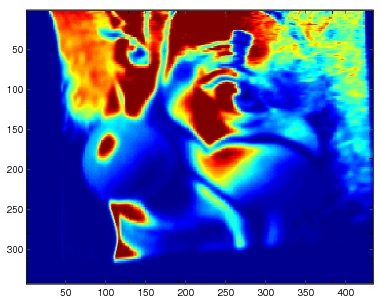
\includegraphics[width=0.8\columnwidth]{25linear.jpg}
\caption{Clown image interpolated 25 times with linear interpolation}
\end{figure}
\begin{figure}[h!]
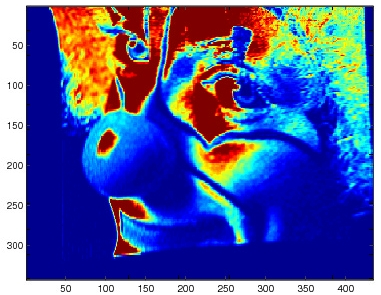
\includegraphics[width=0.8\columnwidth]{25cubic.jpg}
\caption{Clown image interpolated 25 times with cubic interpolation}
\end{figure}
\end{center}

%The main part about interpolation was to understand the existing code and to test it. We were working with cubic interpolation, so, when the number of the sample size double, the error should be divided by $2^4 = 16$.
%We use a very simple test to check this property : we define a function using a product of sinus : $$f(x,y,z) = sin(2\pi m x) * sin(2\pi n y) * sin(2\pi p z)$$
%The parameters $m$, $n$ and $p$ could be changed to make different tests.
%We then generate a huge number $N$ of random points in the grid, compute the interpolation on these points and then evaluate the error by computing the vaue of $f$ in each of these $N$ points.

%The first test was carried out with grids of 32, 64, 128 points and so with spacing of $\cfrac{1}{31}$, $\cfrac{1}{63}$, $\cfrac{1}{127}$. The results were really unexpected and poor :
%\begin{center}
%\begin{tabular}{|c|c|c|c|}
%%  \hline
%  spacing & error & ratio & time \\
%  \hline
%  $\cfrac{1}{31}$ & 0.1038 & 1.0117 &1.773\\[0.2cm] 
%  $\cfrac{1}{63}$ & 0.1026 & 1.5498 &\\[0.2cm]
%  $\cfrac{1}{127}$ & 0.0662 & 1.8807 &\\[0.2cm]
%  $\cfrac{1}{255}$ & 0.0352 &  &\\[0.2cm]
%  \hline
%\end{tabular}
%\end{center}
%The ratio is the one between a grid and the grid with the double number of points. It is expected to approach 16. We see clearly here that the function does not give good results. 
%
%We spent a very large amout of time going through the code and trying to understand what was wrong with the implementation of the cubic interpolation and did not really succeed in it. We finally figure out that the function was only working with ``even'' spacing :
%\begin{center}
%\begin{tabular}{|c|c|c|c|}
%  \hline
%  spacing & error & ratio & time\\
%  \hline
%  $\cfrac{1}{32}$ & 0.0199 & 30.753 &0\\[0.2cm] 
%  $\cfrac{1}{64}$ & 6.471e-4 & 19.966 &\\[0.2cm]
%  $\cfrac{1}{128}$ & 3.241e-5 & 16.965 &\\[0.2cm]
%  $\cfrac{1}{256}$ & 1.91e-6 & & \\[0.2cm]
 % \hline
%\end{tabular}
%\end{center}
%The ratios are approaching 16 much more clearly. We did not fine an explanation for these results, and decided to move on with grids with an ``even'' spacing.


%\subsubsection{Were there several possible implementations?}

%Your text here...

%++++++++++++++++++++++++++++++++++++++++++++++++++++++++++++++++++++++++++++++
%\subsubsection{If there were several possibilities,
%what were the advantages/disadvantages of each? }

%Your text here...

%++++++++++++++++++++++++++++++++++++++++++++++++++++++++++++++++++++++++++++++
%\subsubsection{Which implementation(s) did we do? Why?}

%Your text here...

%++++++++++++++++++++++++++++++++++++++++++++++++++++++++++++++++++++++++++++++
%\subsubsection{What did we implement? -- Include detailed descriptions}

%Your text here...

%++++++++++++++++++++++++++++++++++++++++++++++++++++++++++++++++++++++++++++++
%\subsubsection{What didn't we implement? Why not?}

%Your text here...

%==============================================================================
\subsection{Advection}
\begin{center}
\begin{figure*}[ht]
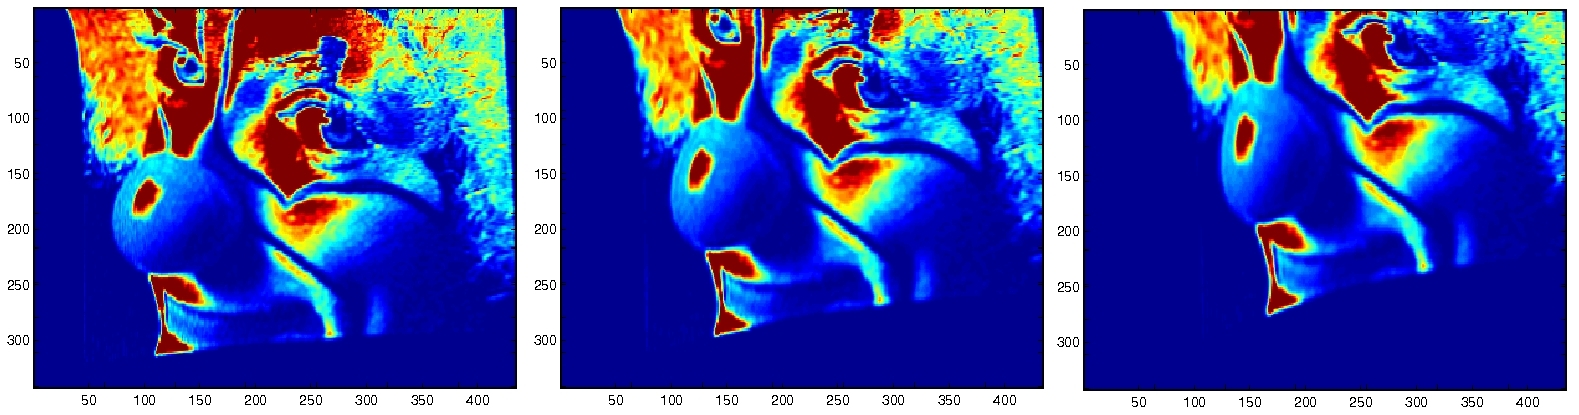
\includegraphics[width = \textwidth]{advect2.jpg}
\caption{Advection at time steps 25, 50, 75 and 100}
\label{advect}
\end{figure*}
\end{center}
%++++++++++++++++++++++++++++++++++++++++++++++++++++++++++++++++++++++++++++++
\subsubsection{Were there several possible implementations?}

The main part of this piece is to implement an integration scheme. Thus there is different possibilities of implementations, such as Euler integration, second order integration or the Runge-Kutta method.

%++++++++++++++++++++++++++++++++++++++++++++++++++++++++++++++++++++++++++++++
\subsubsection{If there were several possibilities,
what were the advantages/disadvantages of each? }

Euler integration is really easy to implement and require just one call to the interpolation function, thus this method would be very fast. Yet, the results would certainly be more blurred than with another method of higher order integration.

In contrast, the Runge-Kutta method will probably be much more accurate, but with 13 calls to the interpolation function, it will probably be much slower than the Euler integration.

%++++++++++++++++++++++++++++++++++++++++++++++++++++++++++++++++++++++++++++++
\subsubsection{Which implementation(s) did we do? Why?}

We choose to implement both Euler and Runge-Kutta integration methods in order to have both quick and accurate results and be able to compare them.

%++++++++++++++++++++++++++++++++++++++++++++++++++++++++++++++++++++++++++++++
\subsubsection{What did we implement? -- Include detailed descriptions}

Advection is about determine the movement of the gridpoints of a given grid $T$ depending on the velocity field. We want, for each gridpoint, to determine its streamline given the velocity field. 

At each time step $dt$, we integrate the velocity field at each grid point, thus we have the points corresponding to the positions of the gridpoints $dt$ ago. Then we interpolate $T$ at these new points and update $T$  with the interpolated values.

The only difference between the two integration methods rely on the way to compute the position of the gridpoints $dt$ ago where to interpolate $T$. 

Indeed, if $X$, $Y$ and $Z$ are the meshgrids containing the coordinates of the gridpoints, and $V_x$, $V_y$, $V_z$ the grids containing the velocity fields, the new positions according to Euler integration would be :

\[
\left\{
\begin{array}{r c l}
X_1 &=& X - dt * V_x\\
Y_1 &=& Y - dt * V_y\\
Z_1 &=& Z - dt * V_z
\end{array}
\right.
\]

For the Runge-Kutta method, we first need to compute the coefficients $k_1$, $k_2$, $k_3$ and $k_4$ for each component : 
\begin{description}
\item[$k_1$] is the values of  $V_x$, $V_y$, $V_z$ at the coordinates $X$,$Y$,$Z$;
\item[$k_2$] at the coordinates
\[
\left\{
\begin{array}{r c l}
X + dt/2 * k_1(x)\\
Y + dt/2 * k_1(y)\\
Z + dt/2 * k_1(z)
\end{array}
\right.
\]

\item[$k_3$] at the coordinates 
\[
\left\{
\begin{array}{r c l}
X + dt/2 * k_2(x)\\
Y + dt/2 * k_2(y)\\
Z + dt/2 * k_2(z)
\end{array}
\right.
\]

\item[$k_4$] at the coordinates 
\[
\left\{
\begin{array}{r c l}
X + dt * k_3(x)\\
Y + dt * k_3(y)\\
Z + dt * k_3(z)
\end{array}
\right.
\]
\end{description}

Then, the new positions where to interpolate $T$ are given by :
\[
\left\{
\begin{array}{r c l}
X_1 \!  &=& \! X + \frac{dt}{6}\left(k_1(x) + 2k_2(x) + 2k_3(x) + k_4(x)\right) \\
Y_1 \!  &=& \! Y + \frac{dt}{6}\left(k_1(y) + 2k_2(y) + 2k_3(y) + k_4(y)\right) \\
Z_1 \!  &=& \! Z + \frac{dt}{6}\left(k_1(z) + 2k_2(z) + 2k_3(z) + k_4(z)\right) 
\end{array}
\right.
\]

Finally, the last step is the same for both Euler and Runge-Kutta methods : interpolate the grid $T$ at the points of coordinates $X_1$, $Y_1$, and $Z_1$, and update $T$ with these new values.

The pictures \ref{advect} is a example of the clown image advected with the Runge-Kutta integration, with a velocity field defined as
\[
\left\{
\begin{array}{r c l}
V_x \!  &=& \! Y \\
V_y \!  &=& \! -X \\
V_z \!  &=& \! 0 
\end{array}
\right.
\]


%At this point of the implementation, we run a test on an image with the cubic interpolation we had tested before. Then we realized this function kept switching the two dimensions $X$ and $Y$, and had a lost of memory leaks : after a few step, Matlab was crashing. We try to understand the cause of the problem and to fix the function and lost again a lot of time. We then decide to use the built-in Matlab function \verb+interp3+, which was giving correct results.
%++++++++++++++++++++++++++++++++++++++++++++++++++++++++++++++++++++++++++++++
%\subsubsection{What didn't we implement? Why not?}

%Your text here...

%==============================================================================
\subsection{Poisson solver}

The last step to solve the incompressible Euler equations is to transform the velocity field $\mathbf{\omega}$ into a divergence-free velocity field $\mathbf{u}$ by solving the Poisson equation :
$$\nabla^2 p = - \mathbf{\nabla} \cdot \mathbf{\omega}   $$
And then, $\mathbf{u}$ is given by $$\mathbf{u}  = {\mathversion{bold}\omega} -  \nabla p$$ 
We want to simulate smoke evolving in a box, we will thus use the Neumann boundary condition $$\mathbf{u} \cdot \mathbf{\hat{n}} = 0  $$
As explain by Alim\cite{alim:ms}, this condition prevent smoke to move orthogonal to the walls.


%++++++++++++++++++++++++++++++++++++++++++++++++++++++++++++++++++++++++++++++
\subsubsection{Were there several possible implementations?}

With our domain as a grid, the Poisson problem is a system of linear equation. There are many methods to solve it \cite{alim:ms,demmel}, some are direct and some other iterative.
For example the conjugate gradient method is iterative and refine a solution at each iteration step until some convergence criterion is satisfy. On the other side, a direct method get an exact solution of the problem in one iteration.

The conjugate-gradient method is practical because it works on every type of domains, though it is often quite expensive. But our domain is rectangular and simple, and thus we will use a rapid fast Fourier transform (FFT) solver.

%++++++++++++++++++++++++++++++++++++++++++++++++++++++++++++++++++++++++++++++
%\subsubsection{If there were several possibilities,
%what were the advantages/disadvantages of each? }

%Your text here...

%++++++++++++++++++++++++++++++++++++++++++++++++++++++++++++++++++++++++++++++
%\subsubsection{Which implementation(s) did we do? Why?}

%Your text here...

%++++++++++++++++++++++++++++++++++++++++++++++++++++++++++++++++++++++++++++++
\subsubsection{What did we implement? -- Include detailed descriptions}

We seek guidance from the work of Alim \cite{alim:ms} to implement the FFT method in 3D : We first compute the 3D discrete cosine transform $\mathbf{\hat{\omega}}$ of the velocity field $\mathbf{\omega}$ using an existing function.
Then, we divide $\mathbf{\hat{\omega}}$ by the sum of the eigenvalues of the matrix describing the second-order central diffrence approximation te the Poisson equation. These eigenvalues are defined as : 
\[
\left\{
\begin{array}{r c l}
\lambda_x \!  &=& \! 2 - 2cos(\cfrac{\pi(j-1)}{M}) ~~ j \in 1..M\\
\lambda_y \!  &=& \! 2 - 2cos(\cfrac{\pi(j-1)}{N}) ~~ j \in 1..N\\
\lambda_z \!  &=& \! 2 - 2cos(\cfrac{\pi(j-1)}{P}) ~~ j \in 1..P
\end{array}
\right.
\]
Where $M$, $N$ and $P$ are the dimensions of $X$, $Y$ and $Z$.
Finally, we compute the inverse cosine transform of $$ \cfrac{\hat{f}}{\lambda_x +\lambda_y +\lambda_z }$$
The result is $p$, and we then deduce $\mathbf{u}$ easily from it.
%++++++++++++++++++++++++++++++++++++++++++++++++++++++++++++++++++++++++++++++
%\subsubsection{What didn't we implement? Why not?}

%Your text here...


%###################################################################@@@@@######

\subsection{Simulation}
To simulate smoke, we need to define the meshgrids $X$, $Y$ and $Z$ for the coordinates, and two grids \verb+density+ and \verb+temp+. The first one, \verb+density+, represents the density of smoke in the grid, while  \verb+temp+ represents the temperature at each gridpoint.

We create a source of smoke : a sphere at the bottom of the grid where the density is set to 100 and the temperature to 100 as well, these two grids are set to 0 everywhere else. We will update this source at every timestep in order to have a continuous flow of smoke.
We then need a velocity field : initially there will be no velocity along the $X$ and $Y$ axis, and an inital value $V_0$ for the smoke's velocity along $Z$. 
The velocity field will then be update at every time step according to the force model.

\subsubsection{Force model}
 Our force model relies on three forces, as explained in the work of Fedkiw et al. \cite{Fedkiw:2001} : the buoyancy, the temperature effect and vorticity confinement.

The buoyancy force describes the natural tendance of smoke to rise : 
$$ f_{buoy} = \alpha * density * \mathbf{z}$$

The temperature effect depends on the difference of temperature between each gridpoint and the ambient temperature, which we have set at $T_{amb} = 25$ : 
$$f_{temp} = \beta(temp-T_{amb})\mathbf{z}$$

Finally, to make the result more realistic, we add a term of vorticity confinement, as explain in Alim and in Fedkiw \cite{alim:ms,Fedkiw:2001}.
Vorticity is defined  as the curl of the velocity field and describes the rotational behaviour of the smoke. That is what cause the swirls and curls of the smoke.
Vorticity confinement has been developed by Fedkiw et al. \cite{Fedkiw:2001}, it locates the area where small vorticity features should be added.
The vorticity of a incompressible flow $\mathbf{u}$ is :
$$\mathbf{\omega} = \nabla \times \mathbf{u}$$

We then computed normalized vorticity location vectors $\mathbf{N}$, they point from lower to higher vorticity concentrations : 
$$ \mathbf{N} = \cfrac{\mathbf{\mu}}{\Vert \mathbf{\mu} \Vert} ~~~~~~~ \mathbf{\mu}=\nabla \Vert \omega \Vert $$

And then the vorticity confinement force is computed as :
$$f_{conf} = \epsilon h (N \times \omega)$$
Where $h$ is the spacing of the grid and $\epsilon$ is a positive parameter used to control the amout of confinement to add.

\subsubsection{The method of projection}
To compute the density and the velocity at each time step, we follow a processus :
\begin{enumerate}
\item Add forces to the velocity fields: buoyancy, temperature and vorticity confinement
\item Advect both density and temerature grids, as well as the velocity fields
\item Make the velocity field divergence free using the Poisson solver
\end{enumerate}

%\subsubsection{Were there several possible implementations?}

%Your text here...

%++++++++++++++++++++++++++++++++++++++++++++++++++++++++++++++++++++++++++++++
%\subsubsection{If there were several possibilities,
%what were the advantages/disadvantages of each? }

%Your text here...

%++++++++++++++++++++++++++++++++++++++++++++++++++++++++++++++++++++++++++++++
%\subsubsection{Which implementation(s) did we do? Why?}

%Your text here...

%++++++++++++++++++++++++++++++++++++++++++++++++++++++++++++++++++++++++++++++
%\subsubsection{What did we implement? -- Include detailed descriptions}


%++++++++++++++++++++++++++++++++++++++++++++++++++++++++++++++++++++++++++++++
%\subsubsection{What didn't we implement? Why not?}

%Your text here...

%==============================================================================
\subsection{BCC implementation}
We did not have time to implement the BCC part. Indeed, we were supposed to use some existing code to implement both Cartesian and BCC parts, but this code contained many errors. We thus spent a large amout of time trying to understand and fix these errors, without success. When we finally try to use it during the advection tests, we realize that the code for cubic interpolation was very slow because of memory leaks, we then decided to use the Matlab built-in function in order to move on.

To implement the BCC grids part, the main steps would be the same than for the Cartesian grids. We would have to implement an interpolation function for BCC grids and then the advection and Poisson parts would follow the same process.

\section{Results}

%==============================================================================
\subsection{How did we measure success?}

I think than despite the fact the BCC part was not implemented, we should talk about partial success. Indeed, we have been able to simulate smoke with good results, and to implement and understand the mathematical methods beyond every steps. 

We have become familiar with those methods and have a much better overview of computer graphics fluid simulation.

%==============================================================================
\subsection{What experiments did we execute?}

We try to compare different methods, for example, we have run two simulations on 2000 time steps, one with Euler integration, and the other one using the Runge-Kutta method. 

We also have run the simulation with and without the vorticity confinement force, in order to have a better understanding of its effect on the smoke's movement.

The simulations showed hereinafter have been executed on grids of size $129 \times 129 \times 385$ with these parameters :
\[
\begin{array}{r c l}
\alpha \!  &=& \! 0.0001\\
\beta \!  &=& \! 0.0000001\\
V_0 \!  &=& \! 0.00001 \\
T_{amb} &=& 25 \\
\epsilon &=& 0.1 \\
dt &=& -0.2 \\
\end{array}
\]

The parameters $\alpha$ and $\beta$ have been chosen in order to give the buoyancy and temperature force an effect visible but not too strong, to have the more realistic result possible. The time step $dt$ have been chosen small enough so the flow of smoke does not broke and its rise is smooth.

In the three simulations, the pictures showed after are 2D slices of the density grid. At each time step, We have render the middle slice of the densoty grid in order to visualize the place with the most smoke.
%==============================================================================
\subsection{Provide quantitative results}

\begin{figure*}
  \begin{center}
    \begin{tabular}{ccccccc}
      \includegraphics[width=0.12\linewidth]{Eulernovort1000cubic/0.jpg} & \includegraphics[width=0.12\linewidth]{Eulernovort1000cubic/6.jpg} & \includegraphics[width=0.12\linewidth]{Eulernovort1000cubic/10.jpg} & 
      \includegraphics[width=0.12\linewidth]{Eulernovort1000cubic/25.jpg} & \includegraphics[width=0.12\linewidth]{Eulernovort1000cubic/40.jpg} & \includegraphics[width=0.12\linewidth]{Eulernovort1000cubic/50.jpg} & 
      \includegraphics[width=0.12\linewidth]{Eulernovort1000cubic/65.jpg} \\

      $t = 0$ & $t = 90$ & $t = 150$ & $t = 375$ & $t = 600$  & $t = 750$ & $t = 975$ \\[0.5cm]
      \includegraphics[width=0.12\linewidth]{Eulervort2000cubic/0.jpg} &  \includegraphics[width=0.12\linewidth]{Eulervort2000cubic/6.jpg}&  \includegraphics[width=0.12\linewidth]{Eulervort2000cubic/10.jpg}
      &  \includegraphics[width=0.12\linewidth]{Eulervort2000cubic/25.jpg} &  \includegraphics[width=0.12\linewidth]{Eulervort2000cubic/40.jpg} &  \includegraphics[width=0.12\linewidth]{Eulervort2000cubic/50.jpg}
      &  \includegraphics[width=0.12\linewidth]{Eulervort2000cubic/65.jpg} \\
      $t = 0$ & $t = 90$ & $t = 150$ & $t = 375$ & $t = 600$  & $t = 750$ & $t = 975$ \\ 
    \end{tabular}
    \caption{Smoke simulation at different time steps. The upper pictures are without vorticity and the lower with.}
    \label{vorttest}
  \end{center}
\end{figure*}

\begin{figure*}
  \begin{center}
    \begin{tabular}{ccccccc}
      \includegraphics[width=0.12\linewidth]{Eulervort2000cubic/0.jpg} &  \includegraphics[width=0.12\linewidth]{Eulervort2000cubic/6.jpg}&  \includegraphics[width=0.12\linewidth]{Eulervort2000cubic/10.jpg}
      &  \includegraphics[width=0.12\linewidth]{Eulervort2000cubic/50.jpg} &  \includegraphics[width=0.12\linewidth]{Eulervort2000cubic/80.jpg} &  \includegraphics[width=0.12\linewidth]{Eulervort2000cubic/110.jpg}
      &  \includegraphics[width=0.12\linewidth]{Eulervort2000cubic/130.jpg} \\
      $t = 0$ & $t = 90$ & $t = 150$ & $t = 750$ & $t = 1200$  & $t = 1650$ & $t = 1950$ \\[0.5cm] 
      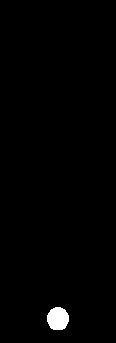
\includegraphics[width=0.12\linewidth]{RKI2000linearvort/0.png} & 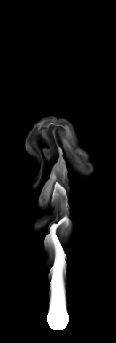
\includegraphics[width=0.12\linewidth]{RKI2000linearvort/6.png} & 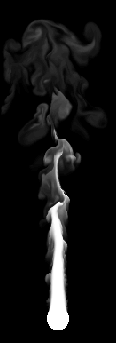
\includegraphics[width=0.12\linewidth]{RKI2000linearvort/10.png} & 
      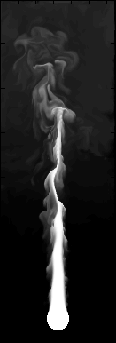
\includegraphics[width=0.12\linewidth]{RKI2000linearvort/50.png} & \includegraphics[width=0.12\linewidth]{RKI2000linearvort/80.png} & \includegraphics[width=0.12\linewidth]{RKI2000linearvort/110.png} & 
      \includegraphics[width=0.12\linewidth]{RKI2000linearvort/130.png} \\

      $t = 0$ & $t = 90$ & $t = 150$ & $t = 750$ & $t = 1200$  & $t = 1650$ & $t = 1950$ \\
    \end{tabular}
    \caption{Smoke simulation at different time steps. The upper pictures are with Euler integration (14s/frame) and the lower with Runge-Kutta (45s/frame), both with vorticity, using cubic interpolation.}
    \label{inttest}
  \end{center}
\end{figure*}
%==============================================================================
\subsection{What do my results indicate?}

The figure \ref{vorttest} shows quite clearly the effect of the vorticity confinement method on the result of the simulation. There are much more little swirls and curls along the smoke flow, and it rise slower.

The figure \ref{inttest} highlights the effect of the integration method use during advection. The results with Runge Kutta integration are more realistic, we see more smoke at the top of the box : there is less dissipation of the smoke. However, the comuptation time difference is not neglectable : the Runge-Kutta advection, with twelve more calls to the interpolation function, takes three times more time that the Euler one.

This is where the BCC grids should be interesting : we expected the same amelioration in results from Cartesian Runge-Kutta to BCC than from Cartesian Euler to Cartesian Runge-Kutta, but the BCC part should not increase the computational time that much. This is the main interrest of BCC grids : better accuracy within the same computational time limits.


%###################################################################@@@@@######
\section{Discussion}

%==============================================================================
\subsection{Overall, is the approach we took promising?}

Our approach is promising since we obtained really realistic results on Cartesian grids using a simple force model and vorticity confinement. The computation time could seems big but we have to keep in mind that our simulations have been runned on high definition grids, which explains that time.

%==============================================================================
\subsection{What different approach or variant of this approach is better?}

The approach using BCC grids should give even better results and reduce the computational time to obtain the same kind of results we get with Runge-Kutta advection and vorticity confinement ;ethod.

%==============================================================================
\subsection{What follow-up work should be done next?}

One of the follow-up work should obviously be the implementation on BCC grids, which would follow the same steps that the approach we have implemented.

Another follow-up work could be to try to render the simulation in 3D to have a better view of the curls and swirls of the smoke.

%==============================================================================
\subsection{What did we learn by doing this project? }

During this project, we have seen ways to use different mathematical methods already known, like the Runge-Kutta intergration for instance, in an applied simulation.

We also have learn other methods such as the Poisson solver.

We also have learn the main steps for fluid simulation in computer graphics, and have a better view of this domain.


%###################################################################@@@@@######
\section{Conclusion}

In conclusion, this project is not a complete success but it still bring us a lot of knowledge about fluid simulation and good results of smoke simulation. Trying to render our results in 3D should be give a very good result, and implementing the same process on BCC grids would improve the quality of our render in the same computational time limits.


%###################################################################@@@@@######
\section*{Acknowledgements}

I would like to thank my supervisor Usman Alim for his patience and his guidance during all steps of this project.

I would also like to thanks the students in the computer graphics lab for their support and the friendly atmosphere of the lab.


%###################################################################@@@@@######
\bibliographystyle{eg-alpha}
\bibliography{refs}

\end{document}
